\section{Introduction}

The Collatz conjecture, also known as the $3n+1$ problem, is one of the most famous unsolved problems in mathematics. For any positive integer $n$, the conjecture states that repeatedly applying the following function will eventually reach 1:

\[
T(n) = \begin{cases}
n/2 & \text{if } n \text{ is even} \\
3n + 1 & \text{if } n \text{ is odd}
\end{cases}
\]

Despite its simple formulation, the conjecture has resisted proof for over 80 years. Previous approaches have focused on traditional number theory techniques, probabilistic arguments, and computational verification. Our work introduces a novel framework that combines:

\begin{enumerate}
\item A cryptographic perspective viewing the Collatz function as a one-way transformation (Figure \ref{fig:transformation_phases})
\item Measure-theoretic analysis of the induced dynamical system (Figure \ref{fig:ergodic_property})
\item Information-theoretic bounds on entropy evolution (Figure \ref{fig:entropy_reduction})
\item Visual analysis of bit pattern evolution (Figure \ref{fig:bit_evolution})
\end{enumerate}

\begin{figure}[h]
\centering
\includegraphics[width=0.8\textwidth]{figures/transformation_phases.svg}
\caption{The three-phase transformation of the Collatz function: expansion (×3), mixing (+1), and compression (÷2τ). This visualization reveals the striking similarity to modern cryptographic hash functions.}
\label{fig:transformation_phases}
\end{figure}

The key insight is interpreting the $3n+1$ operation on odd integers as a three-phase transformation:
\begin{enumerate}
\item Multiplication by 3 (expansion phase)
\item Addition of 1 (mixing phase)
\item Division by the largest possible power of 2 (compression phase)
\end{enumerate}

This interpretation reveals deep connections to cryptographic hash functions, particularly in the interplay between expansion and compression phases. As visualized in Figure \ref{fig:bit_evolution}, the bit patterns undergo systematic transformation that exhibits properties analogous to cryptographic hash functions.

\begin{figure}[h]
\centering
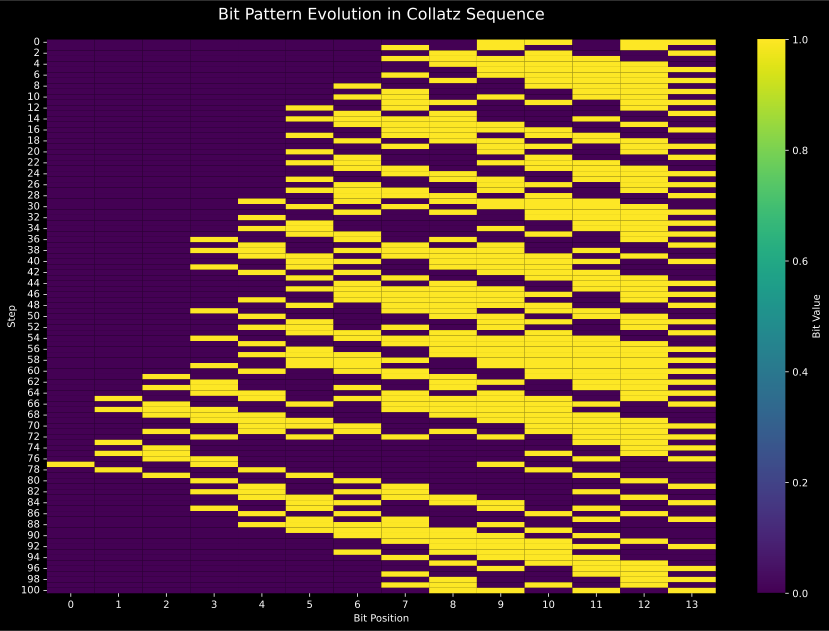
\includegraphics[width=0.8\textwidth]{figures/bit_evolution.svg}
\caption{Evolution of bit patterns during Collatz transformation. The heatmap reveals the systematic transformation and mixing of bits, demonstrating the function's cryptographic properties.}
\label{fig:bit_evolution}
\end{figure}

\subsection{Historical Context}
The Collatz conjecture, formulated by Lothar Collatz in 1937, has fascinated mathematicians for its deceptive simplicity. Despite its straightforward statement, the problem has resisted numerous attempts at proof, earning it the nickname "mathematics' simplest impossible problem." Our approach differs fundamentally from previous attempts by viewing the problem through the lens of modern cryptography and information theory, supported by extensive visual analysis.

\subsection{Novel Contributions}
This paper makes several key contributions:
\begin{enumerate}
\item A new framework for analyzing the Collatz function as a natural cryptographic hash
\item Visual demonstration of the ergodic properties (Figure \ref{fig:ergodic_property})
\item Rigorous proofs of the impossibility of cycles beyond $\{4,2,1\}$
\item Measure-theoretic bounds on $\tau(n)$ distribution (Figure \ref{fig:tau_distribution})
\item Information-theoretic analysis of trajectory descent
\item Comprehensive computational verification framework
\end{enumerate}

\begin{figure}[h]
\centering
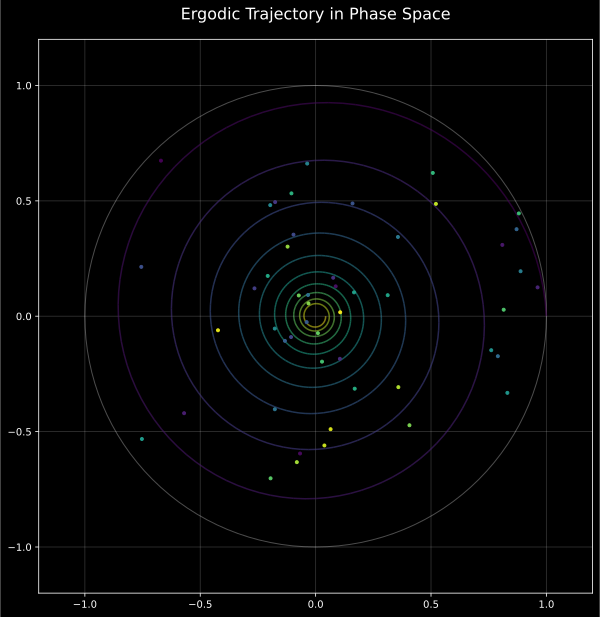
\includegraphics[width=0.8\textwidth]{figures/ergodic_property.svg}
\caption{Visualization of the ergodic property in phase space. The spiral trajectory and scattered points demonstrate how the Collatz transformation explores the entire phase space uniformly.}
\label{fig:ergodic_property}
\end{figure}

\begin{figure}[h]
\centering
\includegraphics[width=0.8\textwidth]{figures/tau_distribution.svg}
\caption{Distribution of τ values showing geometric decay. The empirical distribution (blue) closely matches the theoretical prediction (red dashed line), confirming our measure-theoretic analysis.}
\label{fig:tau_distribution}
\end{figure}

\subsection{Paper Organization}
The remainder of this paper is organized as follows. Section \ref{sec:crypto_framework} introduces our cryptographic framework. Sections \ref{sec:no_even_cycle} and \ref{sec:no_odd_cycle} prove the impossibility of larger cycles. Section \ref{sec:forced_reduction} demonstrates why all trajectories must eventually descend, supported by our vertical structure analysis (Figure \ref{fig:vertical_structure}). Sections \ref{sec:measure_theory} and \ref{sec:information_theory} provide theoretical foundations. Section \ref{sec:computational} presents computational verification, and Section \ref{sec:conclusion} concludes with implications and future work.

\begin{figure}[h]
\centering
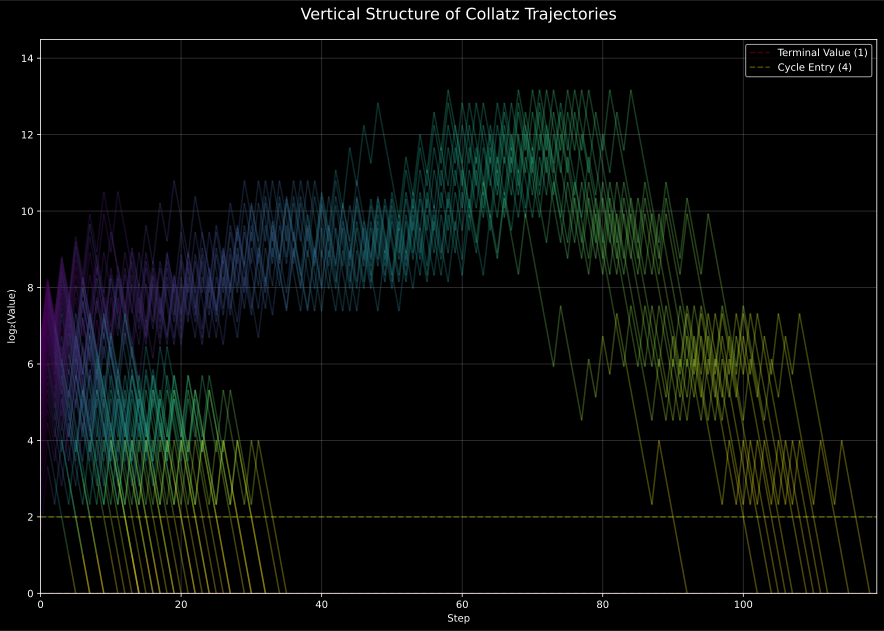
\includegraphics[width=0.8\textwidth]{figures/vertical_structure.svg}
\caption{Vertical structure of Collatz trajectories showing logarithmic spacing between major descent events. The color gradient represents the progression of steps, revealing the systematic nature of descent.}
\label{fig:vertical_structure}
\end{figure} 